\iffalse
\documentclass[journal,10pt,twocolumn]{article}
\usepackage{graphicx, float}
\usepackage[margin=0.5in]{geometry}
\usepackage{amsmath, bm}
\usepackage{array}
\usepackage{booktabs}

\providecommand{\norm}[1]{\left\lVert#1\right\rVert}
\let\vec\mathbf
\newcommand{\myvec}[1]{\ensuremath{\begin{pmatrix}#1\end{pmatrix}}}
\newcommand{\mydet}[1]{\ensuremath{\begin{vmatrix}#1\end{vmatrix}}}

\title{\textbf{Optimization Assignment}}
\author{Pallavarapu Sravan kumar}
\date{October 2022}

\begin{document}

\maketitle
\paragraph{\textit{\large Problem Statement} -
\fi
Find both the maximum value and the minimum value of 
\begin{align}
    f(x) &= 3x^4-8x^3+12x^2-48x+25=0 &  x \in (0,3)
\end{align}
\solution
	\begin{figure}[!ht]
		\centering
		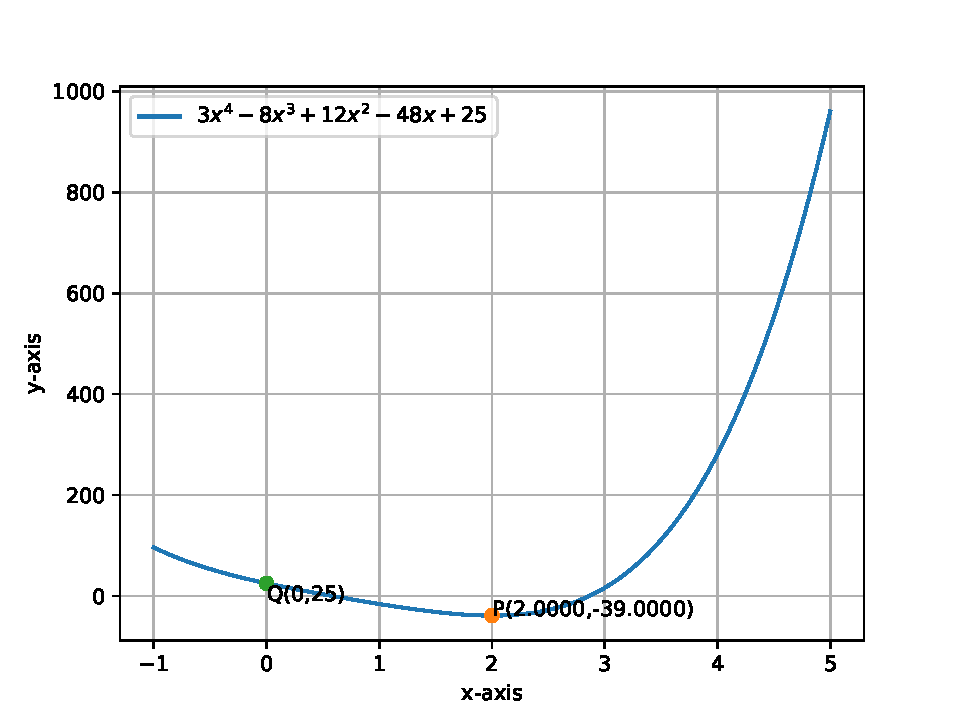
\includegraphics[width=\columnwidth]{12/6/5/7/figs/opt2.pdf}
		\caption{}
		\label{fig:12/6/5/7}
  	\end{figure}
	\iffalse
\section*{\large Figure:}
\begin{figure}[H]
\centering
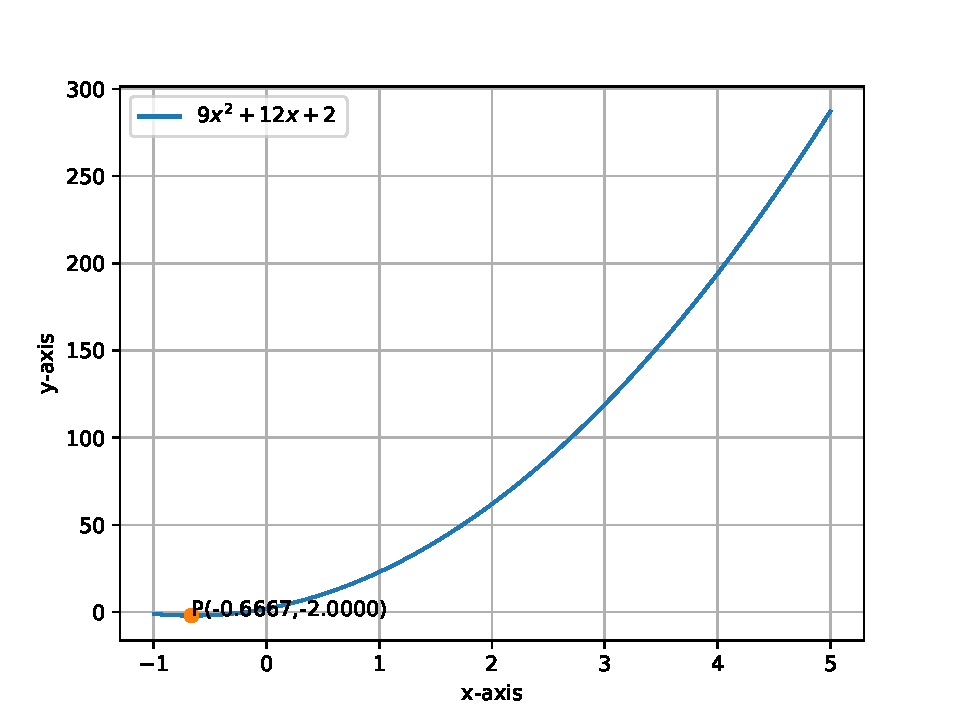
\includegraphics[width=1\columnwidth]{opt2.pdf}
\caption{Graph of f(x)}
\end{figure}



\section*{Solution:}

Given:
\begin{align}
    f(x) &= 3x^4-8x^3+12x^2-48x+25=0 &  x \in (0,3)
\end{align}
\fi
\begin{align}
    \frac{df(x)}{dx} &= 12x^3-24x^2+24x-48
\end{align}
		The minimum can be found using
\begin{align}
        x_{n+1} &= x_n - \alpha \frac{df(x)}{dx}
	\\
          &= x_n - \alpha (12x_n^3-24x_n^2+24x_n-48)
\end{align}
where 
\begin{enumerate}
\item $\alpha$ = 0.001
\item $x_{n+1}$ is current value
\item $x_{n}$ is previous value
\item precession = 0.00000001
\item maximum iterations = 100000000
\end{enumerate}
as
\begin{align}
 	f_{min}= -39\\
 	x_{min}= 2
    \end{align}
    \iffalse
    \item
For maximum, the 
 Critical point is given by
    \begin{align}
       \frac{df(x)}{dx} &= 0 \\
        \implies x &= 2
    \end{align}
    
    and,end points are $x=0$ and $x=3$ .Using table1
    \begin{table}[htbp]
 \begin{center}
    \begin{tabular}{|l|c|c|c|c|c|c} \hline \textbf{x}
  & \textbf{f(x)} \\
 \hline
0 &25\\ \hline
2&-39 \\ \hline
3 &16  \\ \hline	
\end{tabular}   
\end{center}
\caption{Value of f(x)}
\end{table}

 \begin{align}
        \boxed{\text{Maxima} = 25}\\
        \boxed{\text{Maxima Point} = 0}
    \end{align}
   
\end{document}
\fi
